\documentclass[12pt]{article}

\usepackage{amsmath}
\usepackage{array}
\usepackage{caption}
\usepackage[top=1in, bottom=1in, left=0.75in, right=0.75in]{geometry}
\usepackage{graphicx}
\usepackage[colorlinks=true, allcolors=blue]{hyperref}
\usepackage[utf8]{inputenc}
\usepackage{multirow}
\usepackage{pdfpages}
\usepackage[section]{placeins}

\graphicspath{{./figures/}}

\title{ECE 271: Chapter 3 Reading Report}
\author{Phi Luu}
\date{October 15\textsuperscript{th}, 2018}

\begin{document}

\maketitle

%%%%%%%%%%%%%%%%%%%%%%%%%%%%%%%%%%%%%%%%%%%%%%%%%%%%%%%%%%%%%%%%%%%%%%%%%%%%%%%%
% Chapter Outline
%%%%%%%%%%%%%%%%%%%%%%%%%%%%%%%%%%%%%%%%%%%%%%%%%%%%%%%%%%%%%%%%%%%%%%%%%%%%%%%%
\section{Chapter Outline}

This chapter covers the basics of sequential logic design and focuses on the functional and timing relationships between inputs and outputs of a sequential circuit. In this chapter, the authors will show how to build memory for sequential circuits and how to design synchronous logic as well as finite state machines. Finally, like chapter 2, this chapter will finish off with the timing concept and parallelism of sequential logic.

%%%%%%%%%%%%%%%%%%%%%%%%%%%%%%%%%%%%%%%%
% Introduction
%%%%%%%%%%%%%%%%%%%%%%%%%%%%%%%%%%%%%%%%
\subsection{Introduction}

Chapter 2 demonstrates how to analyze and design combinational logic. Recall that the outputs of combinational logic depend \textit{only} on the current value of inputs. \textit{Sequential} logic, on the other hand, has its outputs depending on \textit{both} \textbf{current} and \textbf{previous} input values.

Due to this nature, sequential logic has memory. The memory may explicitly remember the previous inputs or may distill the values into \textit{states} of the system. The state of a digital sequential circuit contains all the necessary past information to explain the future behavior of the circuit. Since memory is an essential component of sequential logic design, latches and flip-flops will be discussed in the following subsection.

%%%%%%%%%%%%%%%%%%%%%%%%%%%%%%%%%%%%%%%%
% Latches and Flip-Flops
%%%%%%%%%%%%%%%%%%%%%%%%%%%%%%%%%%%%%%%%
\subsection{Latches and Flip-Flops}

The fundamental building block of memory is a \textit{bistable} element, an element with two stable states. To further understand what a bistable element looks like, consider Figure~\ref{figure:1}

\begin{figure}[h]
    \centering
    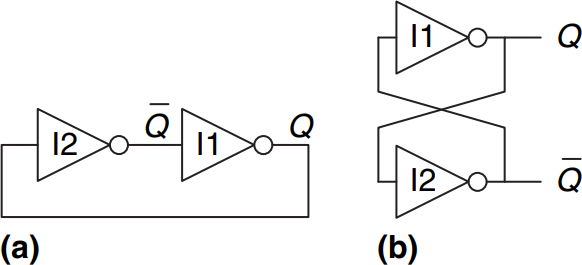
\includegraphics[width=0.5\textwidth]{bistable_elements.png}
    \caption{Cross-coupled inverter pair circuits}
    \label{figure:1}
\end{figure}

The circuits in Figure~\ref{figure:1} do not have any input, instead the output of an inverter is the input of the other inverter. Consider two possible cases for the initial value of $Q$: TRUE and FALSE. Since the circuits are cyclic, one can start from anywhere on the circuits and still go back to the initial position. After going around the circuit, $Q$ still holds the value TRUE if it was initially set to TRUE and still holds the value FALSE if it was initially set to FALSE. Therefore, $Q$ is a bistable element.

When the power is first applied to the circuit, the initial state is unknown and thus becomes unpredictable. The cross-doubled inverters are not practical since the user has no inputs to control the state. There are alternative bistable elements that provide input control: \textit{latches} and \textit{flip-flops}.

\begin{enumerate}
    %%%%%%%%%%%%%%%%%%%%
    % SR Latch
    %%%%%%%%%%%%%%%%%%%%
    \item \textbf{SR Latch}
    \textit{SR latch} is composed of two cross-doubled NOR gates, as shown in Figure~\ref{figure:2}. The latch has two inputs, $S$ and $R$, and has two outputs, $Q$ and $\bar{Q}$.

    \begin{figure}[h]
        \centering
        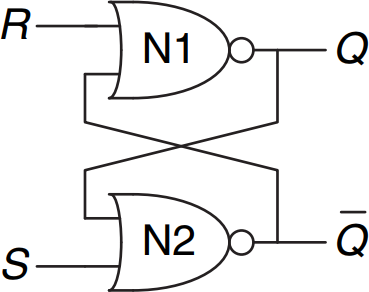
\includegraphics[width=0.25\textwidth]{sr_latch.png}
        \caption{Schematic of an SR latch}
        \label{figure:2}
    \end{figure}

    The truth table of the SR latch can be solved by considering the inputs case by case.

    \begin{enumerate}
        \item $R = 0$, $S = 1$

        When $S = 1$, N2 is always FALSE ($\bar{Q} = \text{FALSE}$). Thus, N1 can be expressed as $R \text{NOR FALSE} = \text{FALSE NOR FALSE} = \text{TRUE}$, and so $Q = \text{TRUE}$.

        \item $R = 1$, $S = 0$

        Similarly to the first case, $Q = \text{FALSE}$ and $\bar{Q} = \text{TRUE}$

        \item $R = 1$, $S = 1$

        $Q = \bar{Q} = \text{FALSE}$, using the same deduction method as the first case.

        \item $R = 0$, $S = 0$

        When $R = S = 0$, the output of N1 depends on the output of N2 and vice versa. Thus, the value of $Q$ and $\bar{Q}$ cannot be solved unless the previous value of $Q$ is known.

        \begin{enumerate}
            \item $Q_{prev} = 0$

            If $Q_{prev} = 0$, the output of N1 must be FALSE, which causes the second input of N2 to be 0. Thus, N2 will produce $\bar{Q} = \text{TRUE}$ as the output. This output matches with N1, since TRUE NOR FALSE = FALSE.

            \item $Q_{prev} = 1$

            Using the same deduction method by going around the circuit, $\bar{Q} = 0$.
        \end{enumerate}

        Combined these two cases, if $R = 0$ and $S = 0$ then $Q = Q_{prev}$ and $\bar{Q} = \bar{Q}_{prev}$.
    \end{enumerate}

    The truth table for the SR latch is shown in Table~\ref{table:1}.

    \begin{table}
        \centering
        \begin{tabular}{ | c | c | c | c | }
        \hline \rule{0em}{1.15em}
        $\mathbf{R}$ & $\mathbf{S}$ & $\mathbf{Q}$ & $\mathbf{\bar{Q}}$ \\ \hline \rule{0em}{1.15em}
        0            & 0            & $Q_{prev}$   & $\bar{Q}_{prev}$   \\ \hline \rule{0em}{1.15em}
        0            & 1            & 1            & 0                  \\ \hline \rule{0em}{1.15em}
        1            & 0            & 0            & 1                  \\ \hline \rule{0em}{1.15em}
        1            & 1            & 0            & 0                  \\ \hline
        \end{tabular}
        \caption{Truth table of the SR latch}
        \label{table:1}
    \end{table}

    For the sake of abstraction and modularity, the SR latch is represented by the symbol in Figure~\ref{figure:3}

    \begin{figure}[h]
        \centering
        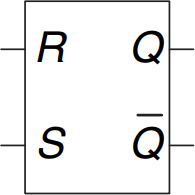
\includegraphics[width=0.125\textwidth]{sr_latch_symbol.png}
        \caption{SR latch symbol}
        \label{figure:3}
    \end{figure}

    The truth table of the SR latch can be interpreted as follows: When R is asserted, the state is set to 0. When S is asserted, the state is set to 1. When both S and R are asserted, the state is set to 0. When neither R nor S is asserted, then the state retains its previous value.

    %%%%%%%%%%%%%%%%%%%%
    % D Latch
    %%%%%%%%%%%%%%%%%%%%
    \item \textbf{D Latch}

    The D latch has two inputs: the \textit{data} input $D$ controlling what the next state should be and the \textit{clock} input $CLK$ controlling when the state should change. $D$ and $CLK$ then interact with each other via two two-input AND gates, and then connect in series with an SR latch, forming the D latch (see Figure~\ref{figure:4}).

    \begin{figure}[h]
        \centering
        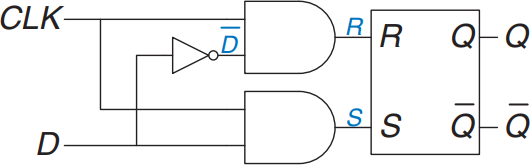
\includegraphics[width=0.3\textwidth]{d_latch_schematic.png}
        \caption{D latch schematic}
        \label{figure:4}
    \end{figure}

    After using the same case-by-case method as the SR latch, the truth table for the D latch is constructed per Table~\ref{table:2} below.

    \begin{table}[h]
        \centering
        \begin{tabular}{ | c | c || c | c | c || c | c | }
        \hline \rule{0em}{1.15em}
        $\mathbf{CLK}$ & $\mathbf{D}$ & $\mathbf{\bar{D}}$ & $\mathbf{R}$ & $\mathbf{S}$ & $\mathbf{Q}$ & $\mathbf{\bar{Q}}$ \\ \hline \rule{0em}{1.15em}
        0              & $X$          & $\bar{X}$          & 0            & 0            & $Q_{prev}$   & $\bar{Q}_{prev}$   \\ \hline \rule{0em}{1.15em}
        1              & 0            & 1                  & 0            & 1            & 0            & 1                  \\ \hline \rule{0em}{1.15em}
        1              & 1            & 0                  & 1            & 0            & 1            & 0                  \\ \hline
        \end{tabular}
        \caption{D latch truth table}
        \label{table:2}
    \end{table}

    The $CLK$ input (or the clock) controls when the data flows through the latch.

    \begin{itemize}
        \item When $CLK = 1$, the latch is \textit{transparent}.

        Data can flow through the latch. $Q = D$.

        \item When $CLK = 0$, the latch is \textit{opaque}.

        Data is blocked from flowing through the latch, thus the output retains its previous value. $Q = Q_{prev}$.
    \end{itemize}

    %%%%%%%%%%%%%%%%%%%%
    % D Flip-Flop
    %%%%%%%%%%%%%%%%%%%%
    \item \textbf{D Flip-Flop}

    A \textit{D flip-flop} (also known as \textit{master-slave flip-flop}, \textit{edge-triggered flip-flop}, \textit{positive edge-triggered flip-flop}) can be built from two back-to-back D latches controlled by complementary clocks, as shown in Figure~\ref{figure:5}. The first latch, $L1$, is called the \textit{master}. The second latch, $L2$, is called the \textit{slave}. The node between $L1$ and $L2$ is named $N1$.

    \begin{figure}[h]
        \centering
        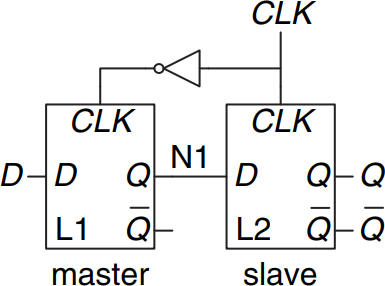
\includegraphics[width=0.3\textwidth]{d_flip_flop_schematic.png}
        \caption{D flip-flop schematic}
        \label{figure:5}
    \end{figure}

    \begin{itemize}
        \item When $CLK = 0$, the master is transparent and the slave is opaque.

        The value at $D$ propagates to the node $N1$ (or $N1 = D$).

        \item When $CLK = 1$, the master is opaque and the slave is transparent.

        The (new) value at $D$ is immediately blocked, and the value at $N1$ propagates to the output $Q$ (or $Q = N1$).
    \end{itemize}

    In short, \textbf{D flip-flop copies D to Q on the rising edge of the clock, and remember its state at all other times.} This is the most important take-out of the D flip-flop.

    Figure~\ref{figure:6} shows the abstract symbol of the D flip-flop. When the $\bar{Q}$ output is not needed, use the minimized symbol on the right.

    \begin{figure}[h]
        \centering
        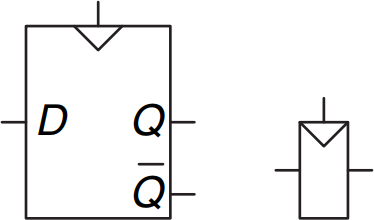
\includegraphics[width=0.25\textwidth]{d_flip_flop_symbols.png}
        \caption{D flip-flop full symbol (left) and minimal symbol (right)}
        \label{figure:6}
    \end{figure}

    %%%%%%%%%%%%%%%%%%%%
    % Register
    %%%%%%%%%%%%%%%%%%%%
    \item \textbf{Register}

    An $N\textit{-bit register}$ is a bank of $N$ flip-flops that share a common $CLK$ input, so that all bits of the register are updated at the same time. Registers are the key building block of most sequential circuits. Figure~\ref{figure:7} shows a 4-bit register and its symbol.

    \begin{figure}[h]
        \centering
        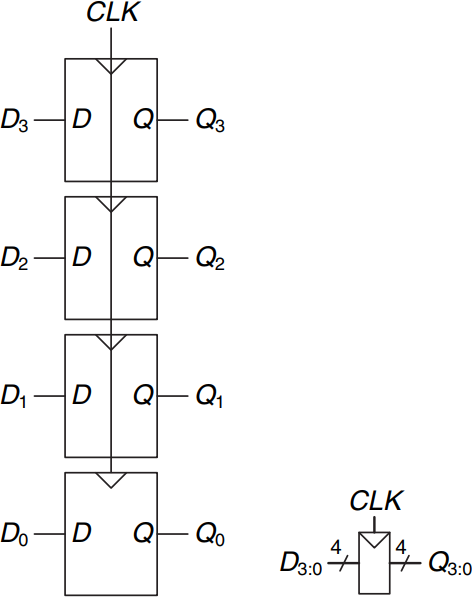
\includegraphics[width=0.25\textwidth]{register_4bit.png}
        \caption{A 4-bit register's schematic (left) and symbol (right)}
        \label{figure:7}
    \end{figure}

    When the register's clock is on ($CLK = \text{TRUE}$), then its $Q$ outputs will change according to their corresponding $D$ inputs. Conversely, the register's $Q$ outputs will retain their previous values if the clock is off ($CLK = \text{FALSE}$).

    %%%%%%%%%%%%%%%%%%%%
    % Enabled Flip-Flop
    %%%%%%%%%%%%%%%%%%%%
    \item \textbf{Enabled Flip-Flop}

    An \textit{enabled flip-flop} is just a flip-flop that has an extra input $EN$ or $\textit{ENABLE}$ to determine whether data can be loaded to the flip-flop.

    \begin{itemize}
        \item When $\textit{EN} = 1 = \text{TRUE}$, an enabled flip-flop behaves just like an ordinary flip-flop, i.e. $Q = Q_{prev}$ if $CLK = 0$ and $Q = D$ if $CLK = 1$.
        \item When $\textit{EN} = 0 = \text{FALSE}$, an enabled flip-flop blocks the incoming data regardless of the $CLK$ value.
    \end{itemize}

    The enabled flip-flop is useful when the user wants to load a new input value only some of the time rather than on every clock edge. Figure~\ref{figure:8} shows the schematics and symbol of the enabled flip-flop.

    \begin{figure}[h]
        \centering
        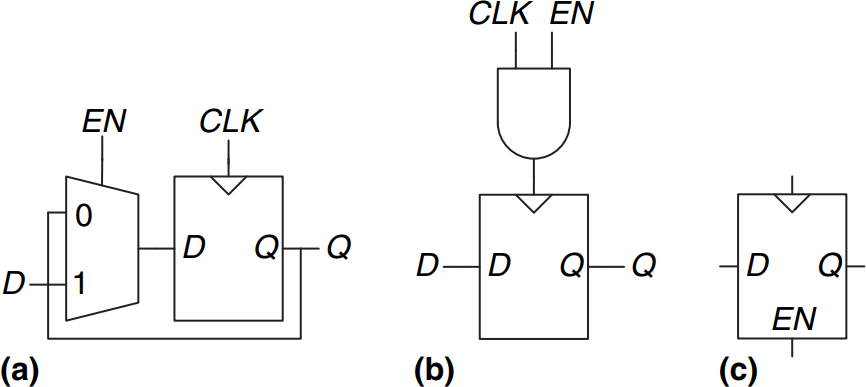
\includegraphics[width=0.45\textwidth]{enabled_flip_flop_schematics_and_symbol.png}
        \caption{The enabled flip-flop schematics (a and b) and symbol (c)}
        \label{figure:8}
    \end{figure}

    %%%%%%%%%%%%%%%%%%%%
    % Resettable Flip-Flop
    %%%%%%%%%%%%%%%%%%%%
    \item \textbf{Resettable Flip-Flop}

    A \textit{resettable flip-flop} is just a flip-flop that has an extra input $\textit{RESET}$.

    \begin{itemize}
        \item When $\textit{RESET} = 1 = \text{TRUE}$, the resettable flip-flop ignores the input $D$ and resets the output $Q$ to 0.
        \item When $\textit{RESET} = 0 = \text{FALSE}$, the resettable flip-flop behaves just like an ordinary flip-flop, i.e. $Q = Q_{prev}$ if $CLK = 0$ and $Q = D$ if $CLK = 1$.
    \end{itemize}

    Resettable flip-flops are useful when the user wants to force a known state (i.e. 0) into all the flip-flops in a system when we first turn it on. Figure~\ref{figure:9} shows the schematics and symbol of the resettable flip-flop.

    \begin{figure}[h]
        \centering
        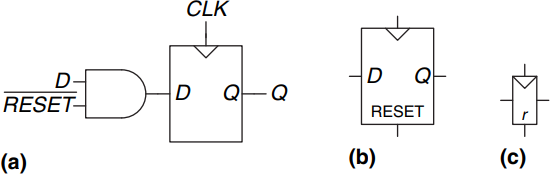
\includegraphics[width=0.5\textwidth]{resettable_flip_flop_schematics_and_symbol.png}
        \caption{The resettable flip-flop schematics (a and b) and symbol (c)}
        \label{figure:9}
    \end{figure}

    %%%%%%%%%%%%%%%%%%%%
    % Transistor-Level Latch and Flip-Flop Designs
    %%%%%%%%%%%%%%%%%%%%
    \item \textbf{Transistor-Level Latch and Flip-Flop Designs}

    The fundamental role of a latch is to be transparent or opaque, like a switch. Since latches and flip-flops require a large amount of transistors to implement when built from logic gates, transmission gates can be used to reduce the hardward needed.

    %%%%%%%%%%%%%%%%%%%%
    % Putting It All Together
    %%%%%%%%%%%%%%%%%%%%
    \item \textbf{Putting It All Together}

    Latches and flip-flops are the fundamental building blocks of sequential circuits. D-latch is level-sensitive, and D flip-flop is edge-triggered.

    D-latch is transparent when $CLK = 1$, allowing $D$ to flow through to $Q$. D flip-flop copies $D$ to $Q$ on the rising edge of $CLK$. At all other times, the outputs $Q$ of both latch and flip-flop retain their previous value (old state).

    A register, which is used in various sequential circuits, is a series of flip-flops, all connected to a single $CLK$ bus.
\end{enumerate}

%%%%%%%%%%%%%%%%%%%%%%%%%%%%%%%%%%%%%%%%
% Synchronous Logic Design
%%%%%%%%%%%%%%%%%%%%%%%%%%%%%%%%%%%%%%%%
\subsection{Synchronous Logic Design}

Sequential circuits are not the same as combinational circuits. The outputs in sequential circuits cannot be determined just by looking at the current values of the inputs. This subsection introduces the notion of synchronous sequential circuits and the dynamic discipline. These concepts will be useful in analyzing and designing sequential circuits.

\begin{enumerate}
    %%%%%%%%%%%%%%%%%%%%
    % Some Problematic Circuits
    %%%%%%%%%%%%%%%%%%%%
    \item \textbf{Some Problematic Circuits}

    The three-inverter loop (Figure~\ref{figure:10}) is an \textit{astable} circuit because the value of $X$ contradicts with its initial value after looping back from $Z$ to $X$.

    \begin{figure}[h]
        \centering
        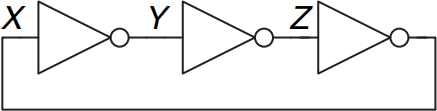
\includegraphics[width=0.25\textwidth]{three_inverter_loop.png}
        \caption{Three-inverter loop}
        \label{figure:10}
    \end{figure}

    An example circuit below (Figure~\ref{figure:11}) is a sequential circuit with a \textit{race condition}. A race condition causes the circuit to fail when some gates are slower than the others. In this case, if the inverter from $CLK$ to $\overline{CLK}$ has a longer delay than the AND and the OR gates, then $Q$ will become stuck at 0. This is an example of \textit{asynchronous} circuit design in which outputs are directly fed back to inputs.

    \begin{figure}[h]
        \centering
        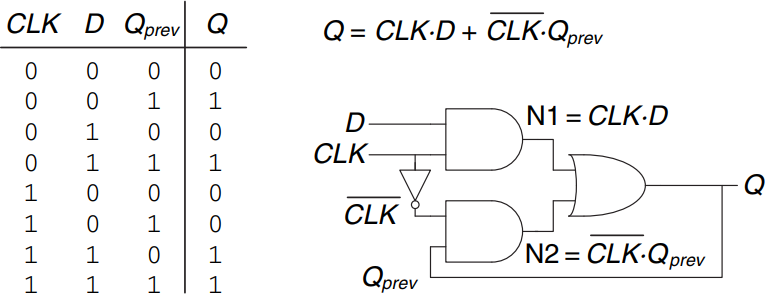
\includegraphics[width=0.5\textwidth]{race_condition_example.png}
        \caption{An asynchronous circuit with a race condition}
        \label{figure:11}
    \end{figure}

    %%%%%%%%%%%%%%%%%%%%
    % Synchronous Sequential Circuits
    %%%%%%%%%%%%%%%%%%%%
    \item \textbf{Synchronous Sequential Circuits}

    To avoid the problems mentioned above, it is recommended to add registers somewhere on the cyclic path in the circuit. Since the registers force the state of the system to change only on clock edge, the state is \textit{synchronized} to the clock. This method eliminates all races.

    The rule of \textit{synchronous sequential circuit composition} states that a circuit is a synchronous sequential circuit if it consists of the interconnected elements such that

    \begin{itemize}
        \item Every circuit element is either a register or a combinational circuit.
        \item At least one circuit element is a register.
        \item All registers receive the same clock signal.
        \item Every cyclic path contains at least one register.
    \end{itemize}

    From these criteria, the flip-flop is the simplest synchronous sequential circuit. Two other common types of synchronous sequential circuit are \textit{finite state machines} and \textit{pipelines}, which will be introduced in the next subsections.

    %%%%%%%%%%%%%%%%%%%%
    % Synchronous and Asynchronous Circuits
    %%%%%%%%%%%%%%%%%%%%
    \item \textbf{Synchronous and Asynchronous Circuits}

    Different from synchronous design, \textit{asynchronous design} is more general since the timing of the system is not blocked by registers (see the example sequential circuits in Figure~\ref{figure:11}). Asynchronous is necessary when communicating between systems with different clock or when receiving inputs at arbitrary times.
\end{enumerate}

%%%%%%%%%%%%%%%%%%%%%%%%%%%%%%%%%%%%%%%%
% Finite State Machines
%%%%%%%%%%%%%%%%%%%%%%%%%%%%%%%%%%%%%%%%
\subsection{Finite State Machines}

[Opening paragraph, if any]

\begin{enumerate}
    %%%%%%%%%%%%%%%%%%%%
    % FSM Design Examples
    %%%%%%%%%%%%%%%%%%%%
    \item \textbf{FSM Design Example}

    %%%%%%%%%%%%%%%%%%%%
    % State Encodings
    %%%%%%%%%%%%%%%%%%%%
    \item \textbf{State Encodings}

    %%%%%%%%%%%%%%%%%%%%
    % Moore and Mealy Machines
    %%%%%%%%%%%%%%%%%%%%
    \item \textbf{Moore and Mealy Machines}


    %%%%%%%%%%%%%%%%%%%%
    % Factoring State Machines
    %%%%%%%%%%%%%%%%%%%%
    \item \textbf{Factoring State Machines}

    %%%%%%%%%%%%%%%%%%%%
    % Deriving an FSM from a Schematic
    %%%%%%%%%%%%%%%%%%%%
    \item \textbf{Deriving an FSM from a Schematic}

    %%%%%%%%%%%%%%%%%%%%
    % FSM Review
    %%%%%%%%%%%%%%%%%%%%
    \item \textbf{FSM Review}
\end{enumerate}

%%%%%%%%%%%%%%%%%%%%%%%%%%%%%%%%%%%%%%%%
% Timing of Sequential Logic
%%%%%%%%%%%%%%%%%%%%%%%%%%%%%%%%%%%%%%%%
\subsection{Timing of Sequential Logic}

[Opening paragraph, if any]

\begin{enumerate}
    %%%%%%%%%%%%%%%%%%%%
    % The Dynamic Discipline
    %%%%%%%%%%%%%%%%%%%%
    \item \textbf{The Dynamic Discipline}

    %%%%%%%%%%%%%%%%%%%%
    % System Timing
    %%%%%%%%%%%%%%%%%%%%
    \item \textbf{System Timing}

    %%%%%%%%%%%%%%%%%%%%
    % Clock Skew
    %%%%%%%%%%%%%%%%%%%%
    \item \textbf{Clock Skew}

    %%%%%%%%%%%%%%%%%%%%
    % Metastability
    %%%%%%%%%%%%%%%%%%%%
    \item \textbf{Metastability}

    %%%%%%%%%%%%%%%%%%%%
    % Synchronizers
    %%%%%%%%%%%%%%%%%%%%
    \item \textbf{Synchronizers}

    %%%%%%%%%%%%%%%%%%%%
    % Derivation of Resolution Time
    %%%%%%%%%%%%%%%%%%%%
    \item \textbf{Derivation of Resolution Time}
\end{enumerate}

%%%%%%%%%%%%%%%%%%%%%%%%%%%%%%%%%%%%%%%%
% Parallelism
%%%%%%%%%%%%%%%%%%%%%%%%%%%%%%%%%%%%%%%%
\subsection{Parallelism}

%%%%%%%%%%%%%%%%%%%%%%%%%%%%%%%%%%%%%%%%
% Summary
%%%%%%%%%%%%%%%%%%%%%%%%%%%%%%%%%%%%%%%%
\subsection{Summary}

%%%%%%%%%%%%%%%%%%%%%%%%%%%%%%%%%%%%%%%%%%%%%%%%%%%%%%%%%%%%%%%%%%%%%%%%%%%%%%%%
% Grey Box Exploration
%%%%%%%%%%%%%%%%%%%%%%%%%%%%%%%%%%%%%%%%%%%%%%%%%%%%%%%%%%%%%%%%%%%%%%%%%%%%%%%%
\section{Grey Box Exploration}

\begin{enumerate}
    %%%%%%%%%%%%%%%%%%%%%%%%%%%%%%%%%%%%%%%%
    % First grey box
    %%%%%%%%%%%%%%%%%%%%%%%%%%%%%%%%%%%%%%%%
    \item The first blurb is on page ...

    %%%%%%%%%%%%%%%%%%%%%%%%%%%%%%%%%%%%%%%%
    % Second grey box
    %%%%%%%%%%%%%%%%%%%%%%%%%%%%%%%%%%%%%%%%
    \item The second blurb is on page ...
\end{enumerate}

%%%%%%%%%%%%%%%%%%%%%%%%%%%%%%%%%%%%%%%%%%%%%%%%%%%%%%%%%%%%%%%%%%%%%%%%%%%%%%%%
% Figures
%%%%%%%%%%%%%%%%%%%%%%%%%%%%%%%%%%%%%%%%%%%%%%%%%%%%%%%%%%%%%%%%%%%%%%%%%%%%%%%%
\section{Figures}

Two figures were selected from this chapter for special recognition. Figure[...] was selected ...

% \begin{figure}[h]
%     \centering
%     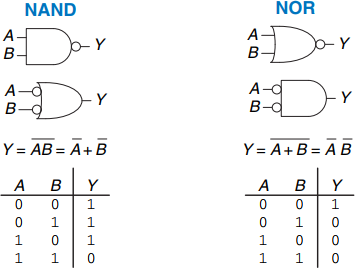
\includegraphics[width=0.5\textwidth]{de_morgan_gates.png}
%     \caption{De Morgan equivalent gates and their truth tables}
%     \label{figure:9}
% \end{figure}

Figure[...] was selected ...

% \begin{figure}[h]
%     \centering
%     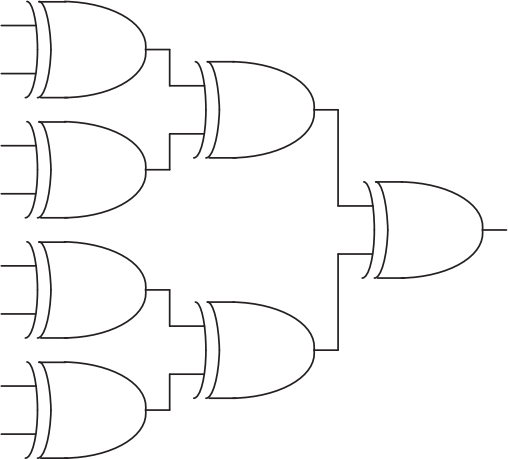
\includegraphics[width=0.25\textwidth]{eight_input_xor}
%     \caption{An eight-input XOR constructed from seven two-input XOR}
%     \label{figure:10}
% \end{figure}

%%%%%%%%%%%%%%%%%%%%%%%%%%%%%%%%%%%%%%%%%%%%%%%%%%%%%%%%%%%%%%%%%%%%%%%%%%%%%%%%
% Example Problems
%%%%%%%%%%%%%%%%%%%%%%%%%%%%%%%%%%%%%%%%%%%%%%%%%%%%%%%%%%%%%%%%%%%%%%%%%%%%%%%%
\section{Example Problems}

See the attached images on the next pages.

% 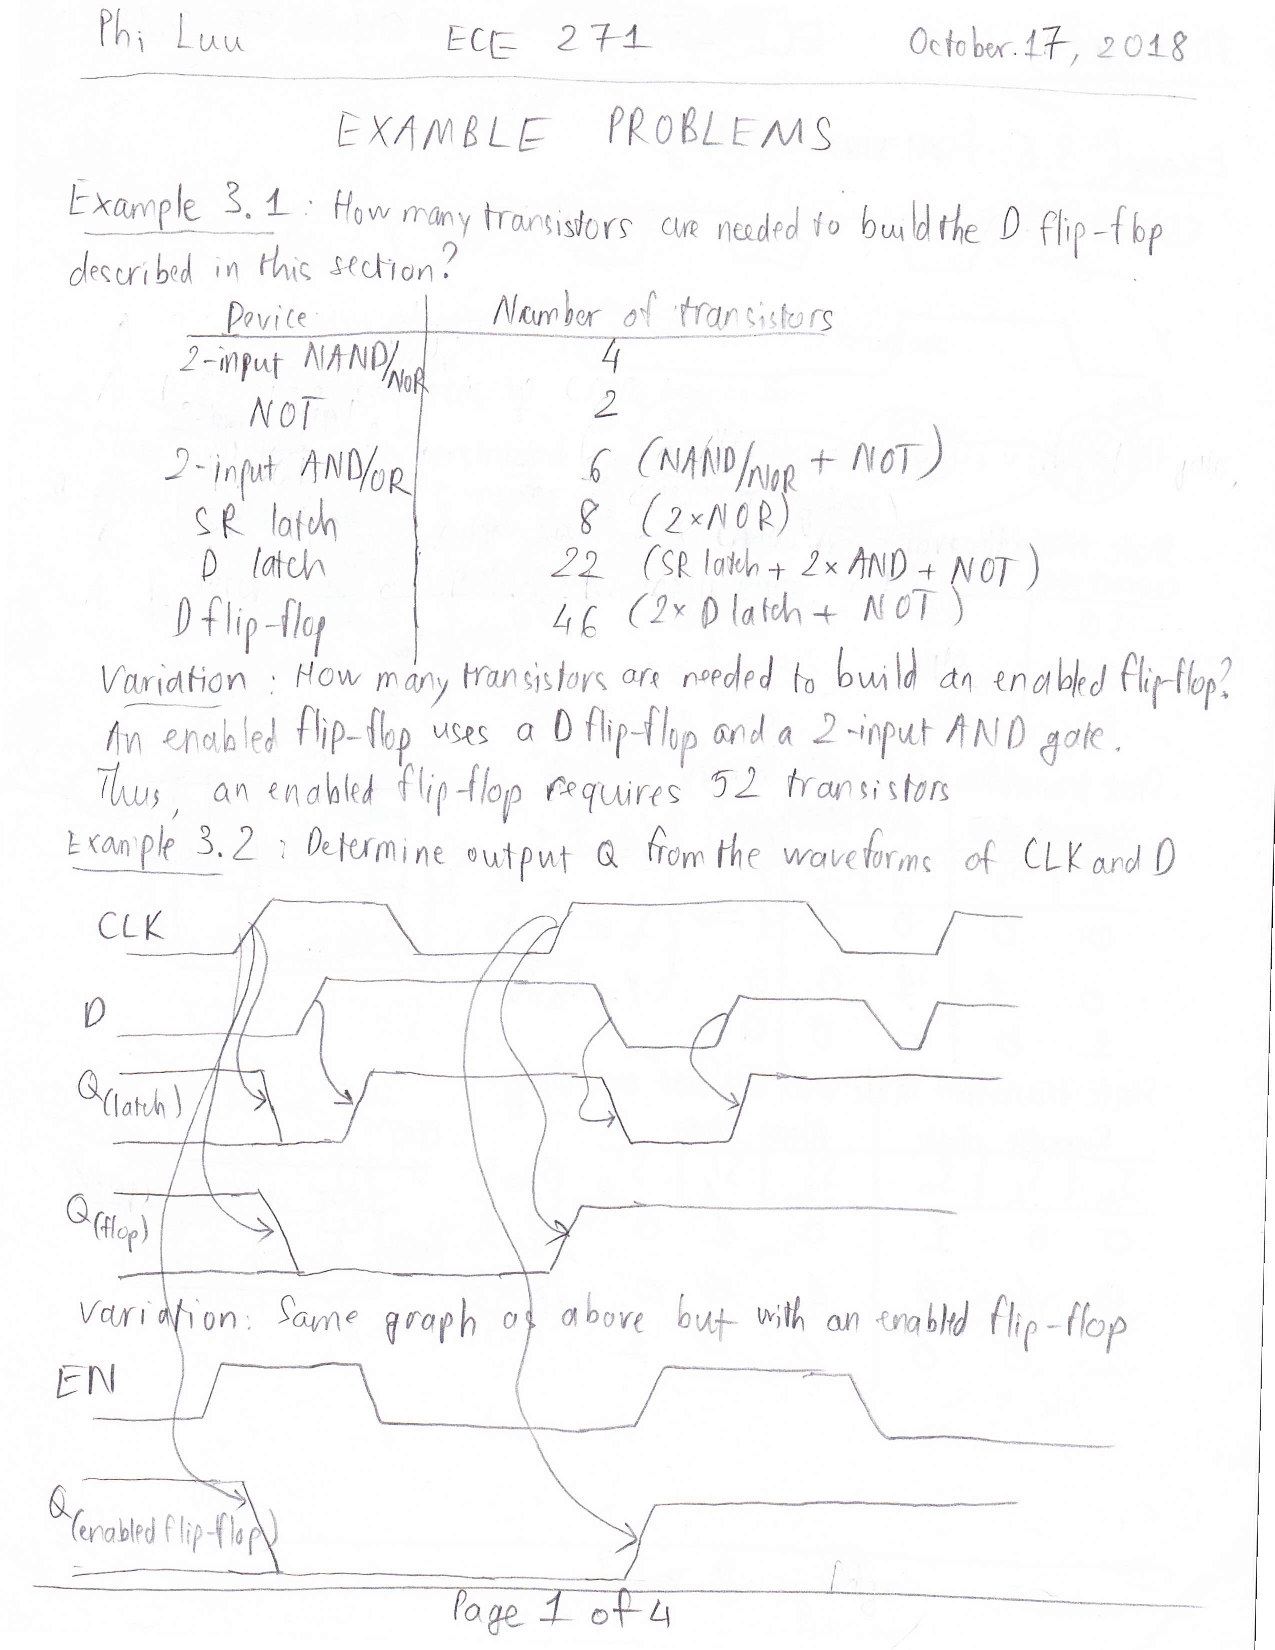
\includepdf[page=-]{example_problems}

%%%%%%%%%%%%%%%%%%%%%%%%%%%%%%%%%%%%%%%%%%%%%%%%%%%%%%%%%%%%%%%%%%%%%%%%%%%%%%%%
% Glossary
%%%%%%%%%%%%%%%%%%%%%%%%%%%%%%%%%%%%%%%%%%%%%%%%%%%%%%%%%%%%%%%%%%%%%%%%%%%%%%%%
\section{Glossary}

All definitions were found from the Google search engine, typing "define state" for the first item.

\begin{enumerate}
    \item State

    noun:

    \begin{enumerate}
        \item the particular condition that someone or something is in at a specific time.
        \item a nation or territory considered as an organized political community under one government.
    \end{enumerate}

    adjective:

    \begin{enumerate}
        \item of, provided by, or concerned with the civil government of a country.
        \item used or done on ceremonial occasions; involving the ceremony associated with a head of state.
    \end{enumerate}

    verb:

    \begin{enumerate}
        \item express something definitely or clearly in speech or writing.
        \item {[music]} present or introduce (a theme or melody) in a composition.
    \end{enumerate}

    \item Sequential

    adjective:

    \begin{enumerate}
        \item forming or following in a logical order or sequence.

        \begin{itemize}
            \item {[computing]} performed or used in sequence.
        \end{itemize}
    \end{enumerate}

    \item{Latch}

    noun:

    \begin{enumerate}
        \item a metal bar with a catch and lever used for fastening a door or gate.
    \end{enumerate}

    verb:

    \begin{enumerate}
        \item fasten (a door or gate) with a latch.
    \end{enumerate}

    \item{Register}

    noun:

    \begin{enumerate}
        \item an official list or record, for example of births, marriages, and deaths, of shipping, or of historic places.
        \item a particular part of the range of a voice or instrument.
    \end{enumerate}

    verb:

    \begin{enumerate}
        \item enter or record on an official list or directory.
        \item (of an instrument) detect and show (a reading) automatically.
    \end{enumerate}

    \item{Flip-Flop}

    noun:

    \begin{enumerate}
        \item a light sandal, typically of plastic or rubber, with a thong between the big and second toe.
        \item {[North American]} a backward handspring.
    \end{enumerate}

    verb:

    \begin{enumerate}
        \item move with a flapping sound or motion.
        \item {[informal $\cdot$ North American]} make an abrupt reversal of policy.
    \end{enumerate}
\end{enumerate}

%%%%%%%%%%%%%%%%%%%%%%%%%%%%%%%%%%%%%%%%%%%%%%%%%%%%%%%%%%%%%%%%%%%%%%%%%%%%%%%%
% Interview Question
%%%%%%%%%%%%%%%%%%%%%%%%%%%%%%%%%%%%%%%%%%%%%%%%%%%%%%%%%%%%%%%%%%%%%%%%%%%%%%%%
\section{Interview Question}

See the attached image on the next page.

% 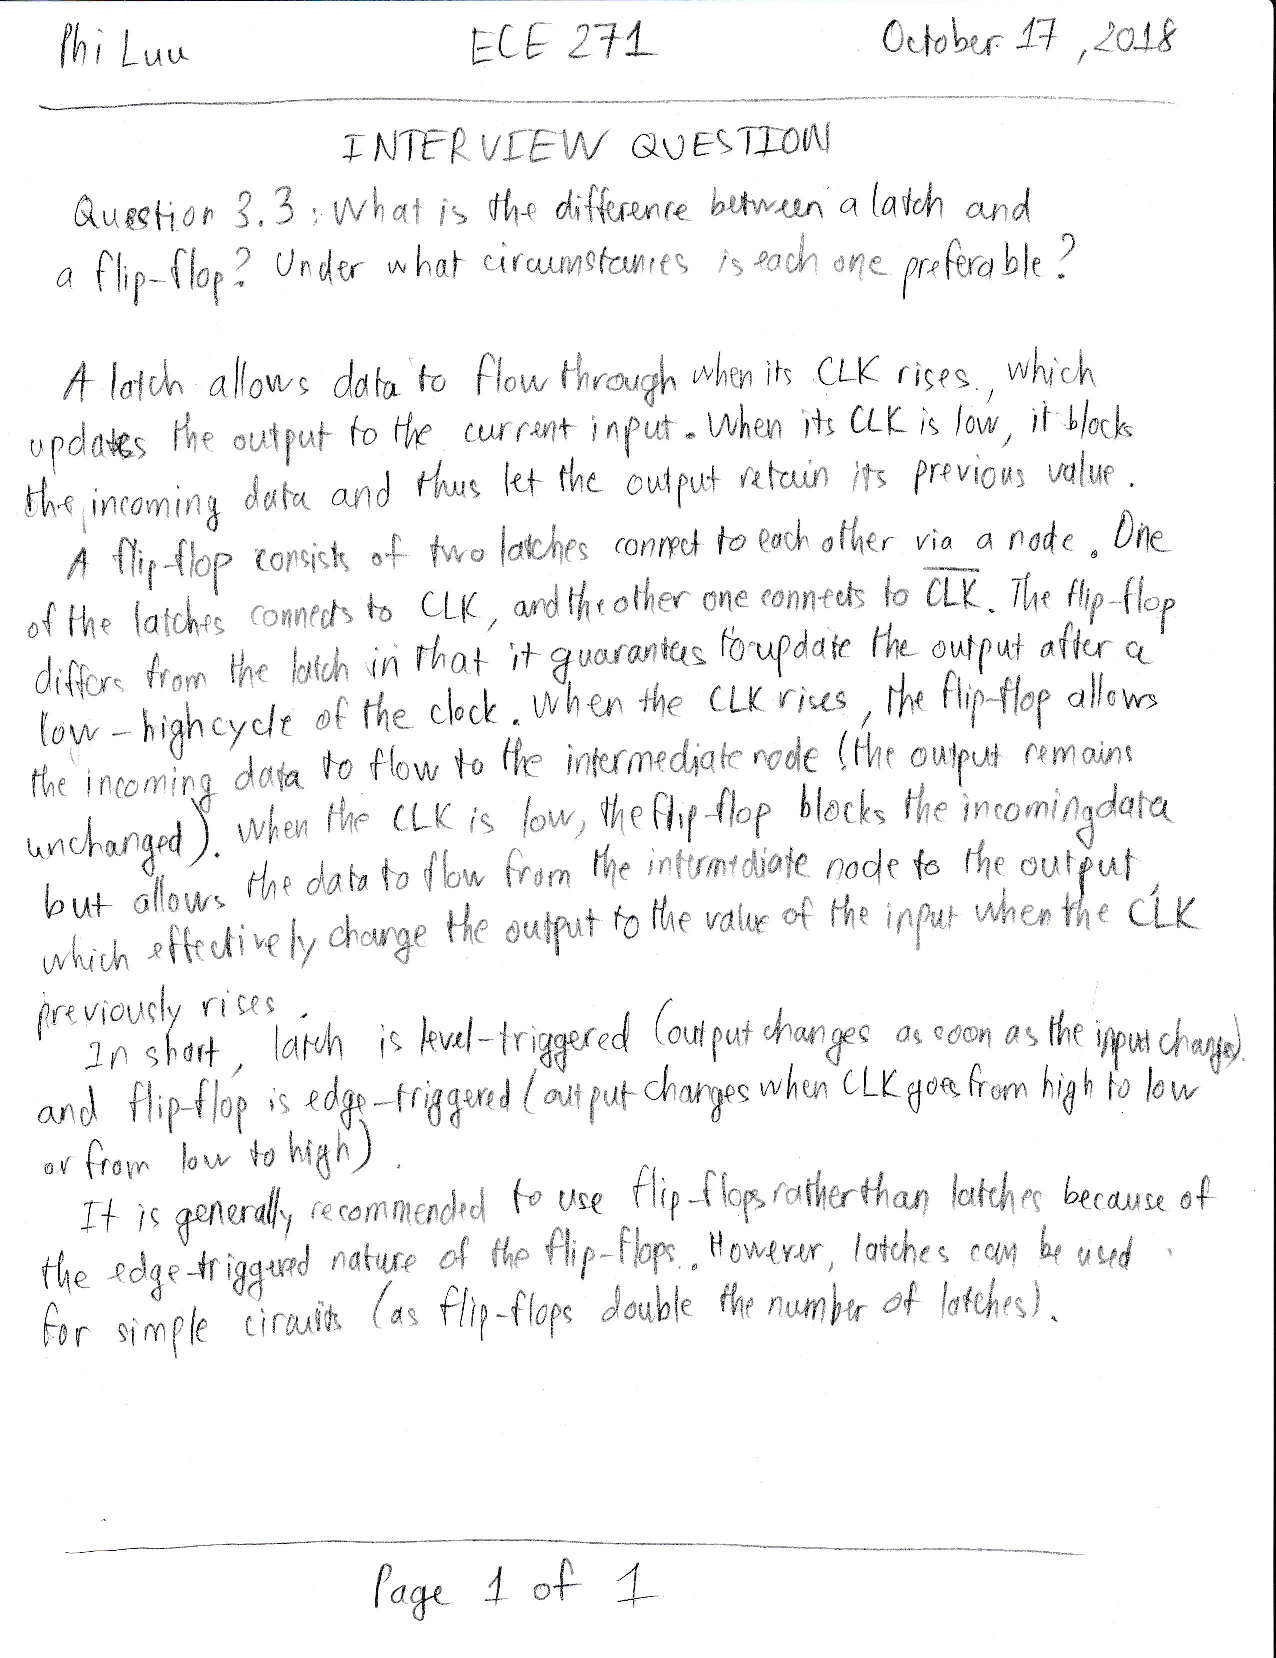
\includepdf[page=-]{interview_question}

%%%%%%%%%%%%%%%%%%%%%%%%%%%%%%%%%%%%%%%%%%%%%%%%%%%%%%%%%%%%%%%%%%%%%%%%%%%%%%%%
% Reflection
%%%%%%%%%%%%%%%%%%%%%%%%%%%%%%%%%%%%%%%%%%%%%%%%%%%%%%%%%%%%%%%%%%%%%%%%%%%%%%%%
\section{Reflection}

%%%%%%%%%%%%%%%%%%%%%%%%%%%%%%%%%%%%%%%%%%%%%%%%%%%%%%%%%%%%%%%%%%%%%%%%%%%%%%%%
% Questions for Lecture
%%%%%%%%%%%%%%%%%%%%%%%%%%%%%%%%%%%%%%%%%%%%%%%%%%%%%%%%%%%%%%%%%%%%%%%%%%%%%%%%
\section{Questions for Lecture}

\begin{enumerate}
    \item QUESTION 1
    \item QUESTION 2
    \item QUESTION 3
\end{enumerate}

%%%%%%%%%%%%%%%%%%%%%%%%%%%%%%%%%%%%%%%%%%%%%%%%%%%%%%%%%%%%%%%%%%%%%%%%%%%%%%%%
% Bibliography
%%%%%%%%%%%%%%%%%%%%%%%%%%%%%%%%%%%%%%%%%%%%%%%%%%%%%%%%%%%%%%%%%%%%%%%%%%%%%%%%
\bibliographystyle{ieeetr}
\bibliography{references}

\end{document}
